\section{Definicion de IA}

\begin{figure}
  \centering
  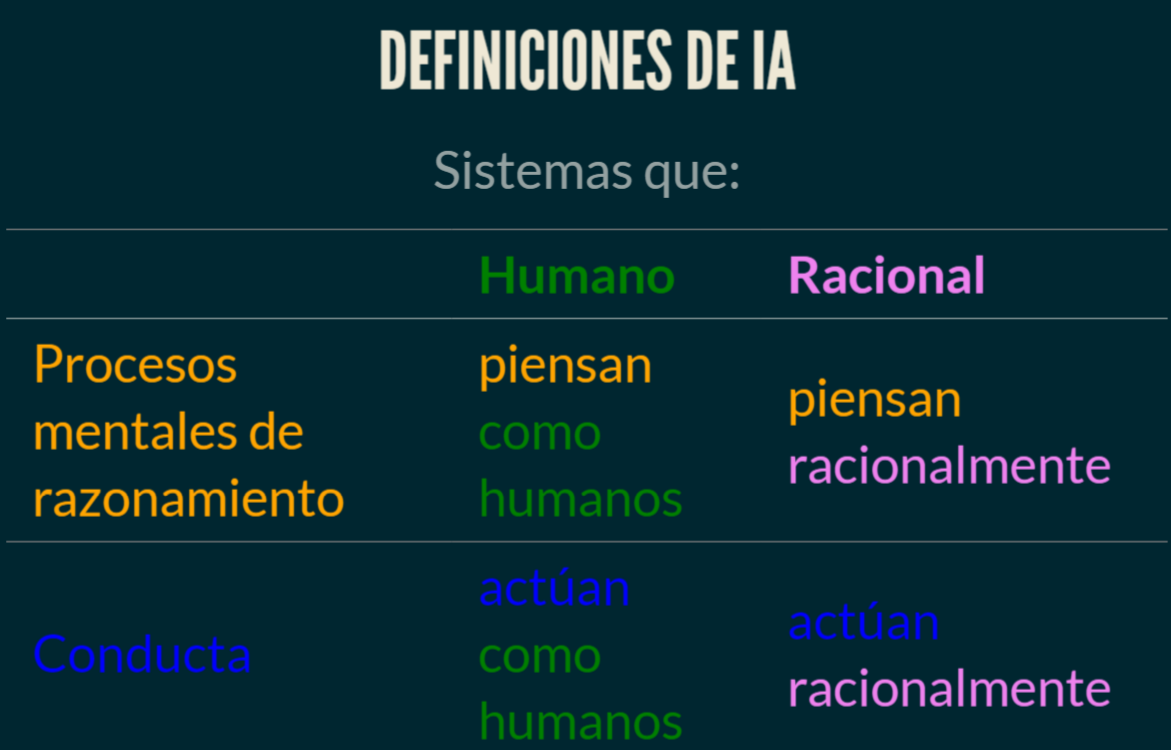
\includegraphics[width=16cm, scale=1]{Images/Imagenes/cuadro1.png}
  \caption{Definiciones de IA}
  \label{fig:marcado}
\end{figure}

\begin{itemize}
  \item \textbf{Piensan como humanos:} Requiere de teorías científicas de las actividades internas del cerebro. Para lograrlo hay que determinar como es que piensan los humanos.
  \item \textbf{Piensan racionalmente:} ir al cap 1 de \cite{sabharwal2011s}
  \item \textbf{Actúan como humanos: }El modelo es el hombre; el objetivo es construir un sistema que se haga pasar por un humano.
  
  Turing propone un Test operacional para el funcionamiento inteligente, las capacidades necesarias son:
  \begin{itemize}
    \item Procesamiento de lenguaje natural
    \item Representación del conocimiento
    \item Razonamiento
    \item Aprendizaje
  \end{itemize}
  El Test consiste en un juez realizando preguntas a dos participantes (X e Y) que no puede ver: un hombre y una mujer. El juez debe averiguar, por medio de preguntas quien es el hombre y quien la mujer. Los participantes pueden mentir o tratar de engañar al juez
  \item \textbf{Actúan racionalmente:} El comportamiento racional hace referencia a realizar la acción correcta. Es decir, aquello que se espera maximice la meta a alcanzar, dada la información disponible
\end{itemize}

\textbf{Agente: }Un agente es una entidad que percibe y actúa. Abstractamente, un agente es una función desde historias de percepciones a acciones:

\begin{equation}
  f: P* \rightarrow A 
\end{equation}

Para toda clase de ambientes y tareas, buscamos el agente con la mejor perfomance